\tikzset{every picture/.style={line width=0.75pt}} %set default line width to 0.75pt        

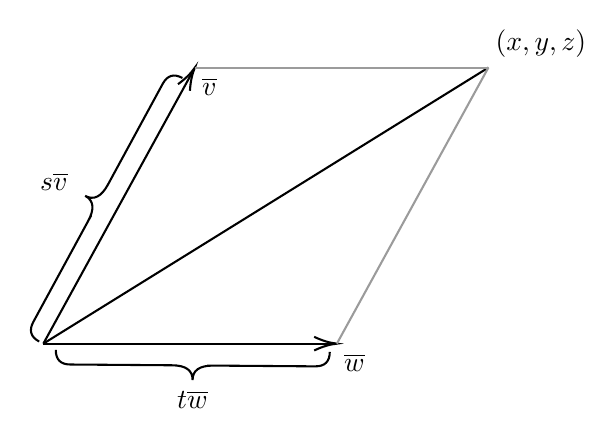
\begin{tikzpicture}[x=0.75pt,y=0.75pt,yscale=-1,xscale=1]
%uncomment if require: \path (0,435); %set diagram left start at 0, and has height of 435

%Straight Lines [id:da890593453199013] 
\draw    (227,151) -- (299.04,19.75) ;
\draw [shift={(300,18)}, rotate = 118.76] [color={rgb, 255:red, 0; green, 0; blue, 0 }  ][line width=0.75]    (10.93,-3.29) .. controls (6.95,-1.4) and (3.31,-0.3) .. (0,0) .. controls (3.31,0.3) and (6.95,1.4) .. (10.93,3.29)   ;
%Shape: Boxed Line [id:dp6624367151910506] 
\draw    (227,151) -- (366.42,151) ;
\draw [shift={(368.42,151)}, rotate = 180] [color={rgb, 255:red, 0; green, 0; blue, 0 }  ][line width=0.75]    (10.93,-3.29) .. controls (6.95,-1.4) and (3.31,-0.3) .. (0,0) .. controls (3.31,0.3) and (6.95,1.4) .. (10.93,3.29)   ;
%Shape: Boxed Line [id:dp16101974014056775] 
\draw    (227,151) -- (441.42,18) ;
%Straight Lines [id:da05231774668964184] 
\draw [color={rgb, 255:red, 155; green, 155; blue, 155 }  ,draw opacity=1 ]   (441.42,18) -- (368.42,151) ;
%Straight Lines [id:da6797188529020097] 
\draw [color={rgb, 255:red, 155; green, 155; blue, 155 }  ,draw opacity=1 ]   (300,18) -- (441.42,18) ;
%Shape: Brace [id:dp39656699893286373] 
\draw   (233,154) .. controls (232.97,158.67) and (235.28,161.02) .. (239.95,161.05) -- (288.95,161.42) .. controls (295.62,161.47) and (298.93,163.83) .. (298.89,168.49) .. controls (298.93,163.83) and (302.28,161.52) .. (308.95,161.57)(305.95,161.55) -- (357.95,161.94) .. controls (362.62,161.97) and (364.97,159.66) .. (365,154.99) ;
%Shape: Brace [id:dp5942404371388796] 
\draw   (294,23) .. controls (289.9,20.77) and (286.74,21.71) .. (284.51,25.81) -- (258.12,74.37) .. controls (254.93,80.23) and (251.29,82.04) .. (247.19,79.81) .. controls (251.29,82.04) and (251.75,86.09) .. (248.57,91.94)(250,89.31) -- (222.18,140.5) .. controls (219.95,144.6) and (220.89,147.76) .. (224.99,149.99) ;

% Text Node
\draw (370.42,154.4) node [anchor=north west][inner sep=0.75pt]    {$\overline{w}$};
% Text Node
\draw (302,21.4) node [anchor=north west][inner sep=0.75pt]    {$\overline{v}$};
% Text Node
\draw (443.42,14.6) node [anchor=south west] [inner sep=0.75pt]    {$( x,y,z)$};
% Text Node
\draw (298.8,172.4) node [anchor=north] [inner sep=0.75pt]    {$t\overline{w}$};
% Text Node
\draw (224,67.4) node [anchor=north west][inner sep=0.75pt]    {$s\overline{v}$};


\end{tikzpicture}
